
\subsection*{Question 1}

La tangente en $A$ est horizontale, donc $f'(-1) = 0$.

\subsection*{Question 2}

On lit sur le graphe que $f'(x) \leq 0$ sur $[-4 ; -1]$ et sur $[1,5 ; 2]$.

\subsection*{Question 3}

On admet que la fonction $f$ est définie sur $[-4 ; 2]$ \\
par $f(x) = (-x^2 + 2,5x - 1)e^x$.\\
La fonction $f$ est un produit de fonctions dérivables sur $[-4 ; 2]$, donc sur cet intervalle :
\begin{align*}
	f'(x) &= (-2x + 2,5)e^x + (-x^2 + 2,5x - 1)e^x \\
	&= e^x \left( -2x + 2,5 - x^2 + 2,5x - 1 \right) \\
	&= e^x (-x^2 + 0,5x + 1,5).
\end{align*}

\subsection*{Question 4}

Le signe de $f'(x)$ dépend du signe du trinôme $-x^2 + 0,5x + 1,5$.\\
Le discriminant de ce trinôme est :
\begin{align*}
	\Delta &= 0,5^2 + 4 \times 1,5 \\
	&= 0,25 + 6 = 6,25 > 0.
\end{align*}
Ce trinôme a donc deux racines :
\begin{align*}
	x_1 &= \frac{-0,5 + 2,5}{-2} = -1, \\
	x_2 &= \frac{-0,5 - 2,5}{-2} = 1,5.
\end{align*}
Le trinôme est négatif sur $[-4 ; -1[$ et sur $[1,5 ; 2]$ et positif sur $[-1 ; 1,5]$.

Ainsi :
\begin{itemize}
	\item $f'(x) < 0$ sur $[-4 ; -1[$ et sur $[1,5 ; 2]$, donc la fonction $f$ est décroissante sur ces intervalles ;
	\item $f'(x) > 0$ sur $[-1 ; 1,5]$, donc la fonction $f$ est croissante sur cet intervalle ;
	\item $f'(-1) = 0$ et $f'(1,5) = 0$, donc $f(-1)$ et $f(1,5)$ sont les extremums de $f$ sur $[-4 ; 2]$.
\end{itemize}

\subsection*{Question 5}

D'après la question précédente, on a le tableau de variations suivant :

\begin{center}
\begin{tikzpicture}
	\tkzTabInit[lgt=3, espcl=3]
	{$x$/1, $f'(x)$/1, $f(x)$/2}
	{$-4$, $-1$, $1.5$, $2$}
	\tkzTabLine{,-,z,+,z,-}
	\tkzTabVar{+/$-27\e^{-4}$, -/$-4.5\e^{-1}$, +/$0.5\e^{4}$, -/$0$}
\end{tikzpicture}
\end{center}

	
